\documentclass[aps,rmp,reprint,superscriptaddress,notitlepage,10pt]{revtex4-1}
\usepackage[utf8x]{inputenc}
\usepackage{amsmath,amsthm,amsfonts,amssymb,amscd}
\usepackage{graphicx}
\usepackage{wrapfig}
\usepackage{enumerate}
\usepackage[final]{hyperref}

\graphicspath{{../figs/}{./figs}}

\begin{document}
%\title{PanGraph: scalable multiple genome alignment for pan-genome analysis}
\title{PanGraph: scalable bacterial pan-genome graph construction}
\author{Nicholas Noll}
\affiliation{Kavli Institute for Theoretical Physics, University of California, Santa Barbara \looseness=-5}
\author{Marco Molari}
\affiliation{Swiss Institute of Bioinformatics, Basel, Switzerland \looseness=-5}
\affiliation{Biozentrum, University of Basel, Basel, Switzerland \looseness=-5}
\author{Richard A.~Neher}
\affiliation{Swiss Institute of Bioinformatics, Basel, Switzerland \looseness=-5}
\affiliation{Biozentrum, University of Basel, Basel, Switzerland \looseness=-5}

\begin{abstract}
    The genomic diversity of microbes is commonly parameterized as population genetic polymorphisms relative to a reference genome of a well-characterized, but arbitrary, isolate.
    Reference genomes contain a fraction of the microbial \emph{pangenome}, the set of genes observed within \emph{all} isolates of a given species, and are thus blind to both the dynamics of the accessory genome, as well as variation within gene order and copy number.
    With the wide-spread usage of long-read sequencing, the number of high-quality, complete genome assemblies has increased dramatically.
    Traditional computational approaches towards whole-genome analysis either scale poorly, or treat genomes as dissociated bags of genes, and thus are not suited for this new era.
    Here, we present \emph{PanGraph}, a Julia based library and command line interface for aligning whole genomes into a graph, wherein each genome is represented as an undirected path along vertices, which in turn, encapsulate homologous multiple sequence alignments.
    The resultant data structure succinctly summarizes population-level nucleotide and structural polymorphisms and can be exported into a several common formats for either downstream analysis or immediate visualization.
\end{abstract}

\maketitle

%\section{Introduction}
During evolution, microbial genomes change by both local modifications and large-scale alterations \cite{arnold2021horizontal}.
Local mutations conserve sequence architecture and only change a few nucleotides by substitution, insertion or deletion.
Conversely, large-scale mutations reorganize the sequence, and involve either the homologous recombination of large segments or wholesale gene loss or gain from the environment.
The accumulation of such polymorphisms over time complicates comparative genomic analyses of present day isolates; microbial genomes are mosaics of homologous sequence, locally related by an asexual phylogenetic tree \cite{sakoparnig2021whole}.
%Scalable inference techniques of this complicated relatedness structure would, in part, spur the advance of critical epidemiological surveillance tools, analogous to NextStrain, for bacterial pathogens.

Recent advances in long-read sequencing have enabled the low-cost assembly of isolated genomes at the quality of reference databases \cite{whibley2021changing}.
The accumulation of many complete genomes promises to rapidly improve our ability to quantify the evolutionary dynamics that drive microbial diversity in natural populations.
Unfortunately, comparative genomic analyses have not kept pace with the technological advance, opting either for reference-based approaches that only partially capture microbial diversity \cite{tettelin2008comparative}  or to construct a \emph{pangenome} that accurately captures nucleotide polymorphisms within genes but approximates structural polymorphisms as simple gene presence-absence relationships \cite{page2015roary,ding2018panx} .
This new era of pangenomics demands novel data structures to encapsulate the \emph{complete} diversity of a given genomic sample set.

In recent years, efforts have focused on generalizing the \emph{pangenome} framework of microbial diversity to graphical models \cite{eizenga2020pangenome}.
At a high level, pangenome graphs generalize the reference sequence coordinate system conventionally used; microbial diversity is, instead, encapsulated by a graph-based data structure, with vertices or edges labelled by homologous DNA sequences, in which a walk recapitulates a subset of mosaic genomes.
As such, pangenome graphs can be thought of as an analogous construct to the well-known assembly graph, in which whole genomes are individual ``reads" of the underlying microbial structure \cite{myers2005fragment}.

While easy to conceptualize, the construction of pangenome graphs has proven computationally challenging.
Colored generalizations of the de Bruijin graph-based assemblers have been successively used to build graphs from large sequence sets, however the underlying efficiency derives from a fixed kmer size which prevents modelling long-range homology \cite{iqbal2012novo,muggli2017succinct}.
An orthogonal approach has been to formulate the inference of the pangenome graph as a multiple genome alignment.
However, current methods either scale poorly to large sets of genomes \cite{darling2010progressivemauve}, focus on comparisons across diverse sets of species across the tree of life at the cost of memory \cite{armstrong2020progressive}, or utilize a reference-guided approach by partitioning genomes first into annotated genes \cite{gautreau2020ppanggolin,colquhoun2021pandora}.

Here we present PanGraph, a Julia \cite{bezanson2017julia} library and command line interface, designed to efficiently align large sets of closely related genomes into a pangenome graph on personal computers.
The resulting graph both compresses the input sequence set and succinctly captures the population diversity at multiple scales ranging from nucleotide mutations and indels to structural polymorphisms driven by inversions, rearrangements, and gene gain/loss.
The underlying graph data structure can be exported into numerous formats for downstream analysis and visualization in software such as Bandage \cite{wick2015bandage}.
%The algorithm, along with extensive documentation, examples, and instructions for installation, are open source and can be found on GitHub.
%We anticipate PanGraph to be immediately useful in understanding microbial evolution in natural populations.

\section{Algorithms and implementation}
\emph{PanGraph} transforms an arbitrary set of genomes into a \emph{graph} that simultaneously compresses the collection of sequences and exhaustively summarizes both the structural and nucleotide-level polymorphisms.
The graph is composed of \emph{pancontigs}, which represent linear multiple-sequence alignments of homologous sequence found within one or more input genomes.
\emph{Pancontigs} are connected by an edge if they are syntenic on at least one input sequence; individual sequences are then recapitulated by contiguous \emph{paths} through the graph.

\emph{PanGraph's} overarching strategy is to approximate multiple-genome alignment by iterative pairwise alignment, in the spirit of progressive alignment tools \cite{darling2010progressivemauve,armstrong2020progressive}.
A guide tree is utilized to linearize the problem's complexity by approximating multiple-sequence alignment as a quenched order of successive pairwise alignments \cite{feng1987progressive}.
Pairwise graph alignment is performed by an all-to-all alignment of the \emph{pancontigs} between both graphs.

\subsection{Guide tree construction}
The alignment guide tree is constructed subject to three design constraints: (i) sequences are aligned sequentially based upon similarity, (ii) the similarity computation scales sub-quadratically with the number of input sequences, and (iii) the resultant tree is balanced.
To this end, we formulate the algorithm as a two step process.
The initial guide tree is constructed by neighbor-joining \cite{saitou1987neighbor}; the pairwise distance between sequences is approximated by the Jaccard distance between sequence minimizers \cite{roberts2004reducing}.
Computationally, each sequence can be sketched into its set of minimizers in linear time while the cardinality of all pairwise intersections can be computed by sorting the list of all minimizers to efficiently count overlaps.
Hence, the pairwise distance matrix is estimated in log-linear time.
The final guide tree is constructed as the balanced binary tree constrained to reproduce the topological ordering of leaves found initially.
See Fig \ref{fig:visualization}A for a graphical depiction of the guide tree.

\subsection{Iterative graph alignment}
The iterative pangraph construction is illustrated in Fig.~\ref{fig:visualization}.
The pangraph is initialized as one subgraph per input genome, each representing its respective genome as a single \emph{pancontig}.
Pairs of subgraphs are aligned in a postorder traversal of the constructed guide tree.
The identified homologous intervals of the pancontig are then merged, thereby creating shorter contigs that represent homologous sections of multiple input genomes, see Fig. \ref{fig:visualization}B for a graphical deption.
These steps of pairwise graph alignment and merging of homologous intervals are repeated until the root of the guide tree is reached.

\paragraph{Pairwise alignment.}
Full genome alignment between two closely related isolates is a well-studied problem with many high-quality tools available \cite{li2018minimap2,marccais2018mummer4}.
We chose to use \emph{minimap2} as the core pairwise genome aligner for its proven speed, sensitivity, and easy-to-use exposed library API \cite{li2018minimap2}.
This alignment kernel is included within a custom Julia wrapper, available at \url{github.com/nnoll/minimap2_jll.jl}.
However, we note that \emph{PanGraph} is written to be modular, and additional alignment kernels can be added with ease.
In particular we decided to include the option to use \emph{mmseqs2} \cite{steinegger2017mmseqs2} as an alternative alignment kernel, because of its sensitivity on highly diverged sequences at the cost of higher computational time.
In general, the kernel interface expects two lists of \emph{pancontigs} to align as input and will output a list of putative overlapping alignments between both input lists.

\paragraph{Merging of homologous sequence.}
\emph{Pancontigs} encapsulate linear multiple-sequence alignments which are modelled internally by a star phylogeny, i.e. are assumed to be well-described by a reference sequence augmented by independent SNPs and indels for each contained isolate.
Importantly, during the all-to-all alignment phase, \emph{pancontigs} are aligned based \emph{solely} upon their consensus sequence.
All putative homologous alignments found by \emph{pancontig} alignment are ranked according to the pseudo-energy
\begin{equation}
    E = -\ell + \alpha N_c + \beta N_m
\end{equation}
where $\ell$, $N_c$, and $N_m$ denote the alignment length, number of \emph{pancontigs} created by the merger, and number of polymorphisms per genome in the newly created {pancontig} respectively.
See Fig \ref{fig:visualization}B for a graphical definition for each term.
Additionally, $\alpha$ and $\beta$ are hyperparameters of the algorithm, respectively controlling the tradeoff between fragmentation of the graph and the maximum diversity within each block.
Only alignments with negative pseudo-energy are performed.

\begin{figure}[htb]
    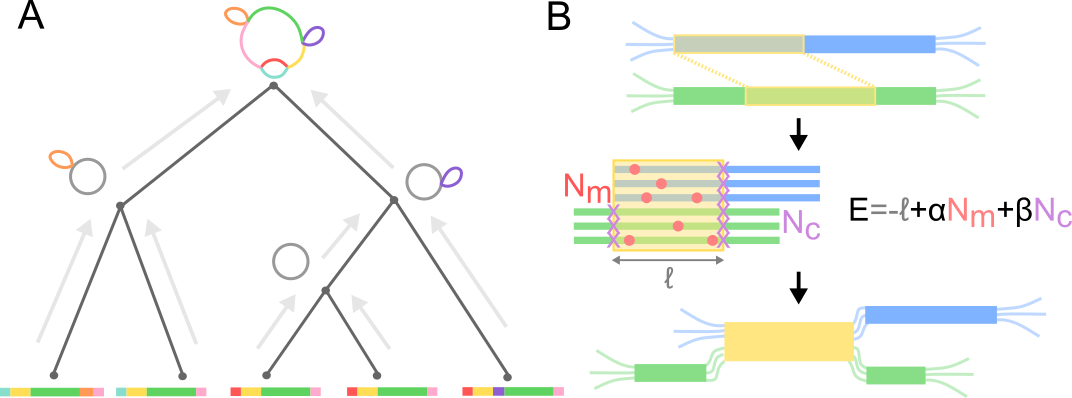
\includegraphics[width=.5\textwidth]{figs/algorithm.png}
    \caption{{\bf Overview of PanGraph algorithm}.
        (A) The alignment graph is constructed progressively by aligning graphs pairwise up a guide tree constructed from neighbor-joining the minimizer overlap between strains.
        (B) During pairwise alignment, \emph{pancontigs} (blue and green)
        are merged by identifying homologous intervals (shown in yellow).
        If the underlying alignments are viewed compatible, i.e. the energy is less than 0, the pancontigs are merged.
    }
    \label{fig:visualization}
\end{figure}

At the graph level, the merger of two \emph{pancontigs} defines a new \emph{pancontig}, connected on both sides by edges to the neighboring \emph{pancontigs} of both inputs, and thus locally collapses the two graphs under consideration.
At the nucleotide level, the pairwise alignment of two \emph{pancontigs} maps the reference of one onto the other; the merger of two \emph{pancontigs} requires the application of the map onto the underlying multiple-sequence alignment.
Once both sets of sequences are placed onto a common coordinate system, the resultant consensus sequence, and thus polymorphisms, are recomputed.
This procedure can be viewed as an online multiple sequence alignment algorithm.

The above procedure is repeated until no alignments with negative energy remain.
Upon completion, transitive edges within the graph are removed by merging adjacent \emph{pancontigs}.

\subsection{Parallelism}
\emph{PanGraph} is designed with a message-passing architecture to enable scalable parallelism, as shown in Fig \ref{fig:visualization}A for a cartoon example.
Each internal node of the guide tree represents a job that performs a single pairwise graph alignment between its two children.
The process will block until both of its children processes have completed and subsequently pass the result of their pairwise graph alignment up to the parent.
All jobs run concurrently from the start of the algorithm; the Julia scheduler resolves the order of dependencies naturally \cite{bezanson2017julia}.
As such, the number of parallel computations is automatically scaled to the number of available threads allocated by the user at the onset of the alignment.

\subsection{Graph Export and Availability}
The constructed pangenome graph can be exported in a variety of file formats for downstream analysis and visualization.
In addition to a custom JSON schema, PanGraph can export the alignment as a GFA file, where each \emph{pancontig} is represented as a segment and each genome as a path.
This allows for visualization in software such as Bandage \cite{wick2015bandage}.
Lastly, we provide functionality to export as a conventional pangenome, however wherein \emph{pancontigs} supplant putative gene clusters, that can be visualized directly by the PanX toolkit \cite{ding2018panx}.

PanGraph is published under an MIT license with source code, extensive documentation, examples, and instructions for installation available at \url{github.com/neherlab/pangraph}.
Additionally, pre-built binaries are available as GitHub releases.
All data and scripts used to validate PanGraph are available within the same repository.

\section{Validation and performance}

\subsection{Validation on synthetic data}

In order to assess the accuracy of the pangenome graph inferred by PanGraph, and to quantify its performance characteristics as a function of input size, we generated synthetic data.
Specifically, we simulated populations of size $N=100$ and sequence length $L=50000$ utilizing a Wright-Fisher model \cite{hudson2002generating} evolved for $T=50$ generations.
In addition to nucleotide mutations that occur at rate $\mu$ per generation, we modelled inversions, deletions (each with independent rates set to $10^{-2}$ per generation), and horizontal sequence transfer that occurs with tunable rate $r$ per generation per genome.
The ancestral state for each sequence is tracked through each evolutionary event so that the true mosaic relatedness structure can easily be converted to a graph.
The simulation framework is distributed within the PanGraph command line toolsuite for external use.


\begin{figure}[htb]
    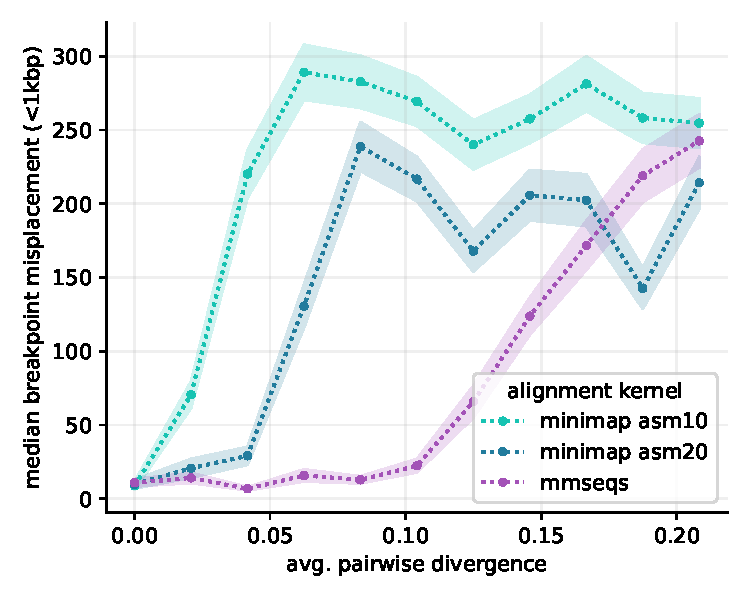
\includegraphics[width=.4\textwidth]{figs/median_misplacement_vs_divergence.pdf}
    \caption{{\bf Accuracy against synthetic data}}
    \label{fig:toy-accuracy}
\end{figure}

We quantified the accuracy of PanGraph algorithm by computing the distance, $\delta$, of the inferred breakpoints relative to their known locus stored from the evolutionary simulation.
Critically, we found that the accuracy was \emph{independent} of the rate of horizontal gene transfer $r$ and thus underlying graph complexity.
The predominant determinant of accuracy was the sample diversity, shown in Fig. \ref{fig:toy-accuracy} which displays the distributions of $\delta$ for $100$ independent simulations ran for each mutation rate $\mu$.
For approximately clonal populations, $\sim 80\%$ of breakpoints were estimated to be within $10$bp away from the ``true" location.
Conversely, for samples with average pairwise diversity above $2\%$, $\sim 80\%$ of breakpoints are estimated only within $100$ bp.
This limitation is primarily driven by lack of sensitivity in the pairwise alignment phase performed using \emph{minimap2} \cite{li2018minimap2}.

\begin{figure}[htb]
    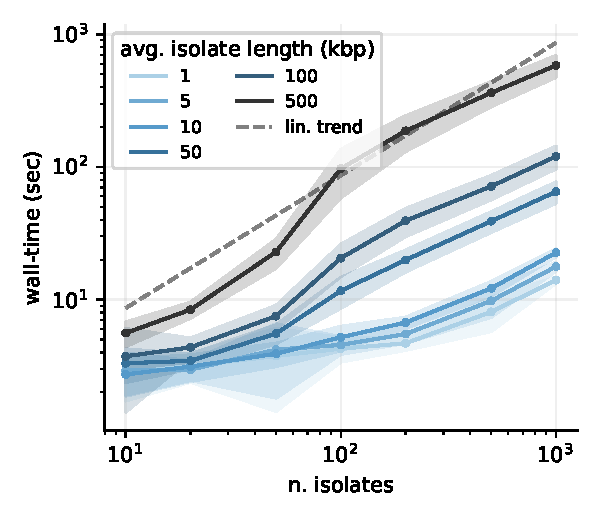
\includegraphics[width=.4\textwidth]{figs/benchmark.pdf}
    \caption{{\bf Algorithm performance}.
        PanGraph scales linearly with the number of input genomes.
        This is a direct result of the guide tree simplification.
        The solid line and ribbons display the mean and standard deviation respectively.
        All runs were performed on an AMD Ryzen 7 2700X utilizing 8 cores.
    }
    \label{fig:toy-performance}
\end{figure}


The algorithmic complexity was measured empirically by simulating populations of increasing size and average sequence length.
The mean and standard deviation of results obtained from 50 iterations are shown in Fig. \ref{fig:toy-performance}.
Importantly, PanGraph's computational complexity grows \emph{linearly} with the number of input genomes.
We note that the PanGraph scales approximately log-linear with average sequence length, as expected from the underlying algorithmic complexity of Minimap2 \cite{li2018minimap2}.

\subsection{Validation on real data}

We additionally validated PanGraph on natural populations sampled from RefSeq \cite{o2016reference}.
Obviously the ``true" breakpoints are not known \emph{a priori} and thus the direct analog of Fig. \ref{fig:toy-accuracy} is not possible.
However, we postulate that most \emph{bona fide} breakpoints generated from evolutionary events will happen at or near gene boundaries; there is preliminary evidence for this assumption \cite{oliveira2017chromosomal}.
We compared the empirical distribution of distances to gene boundaries to a null distribution generated from the data, in which breakpoints are sampled uniformly from each genome, constrained to produce equivalent number of partitions as was measured by PanGraph.
For all tested cases, we find our boundaries cluster closer to genes than would be expected by chance.
The median distance from a Pangraph boundary to annotated gene ranges between 50-100 bp, depending on the species, while the random breakpoint is, on average, 600 bp off.


\begin{figure*}[htb]
    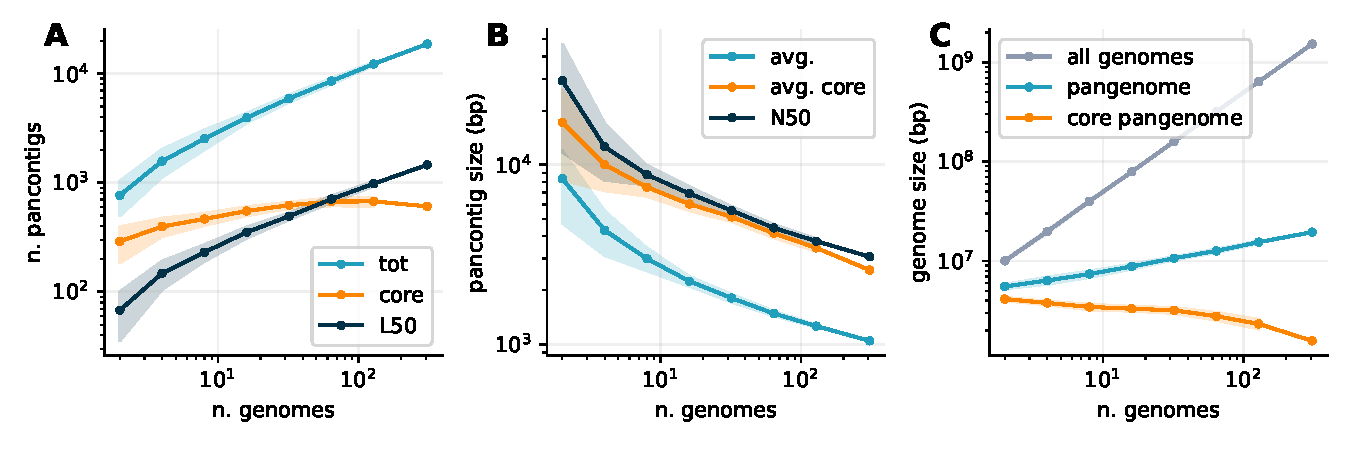
\includegraphics[width=.8\textwidth]{figs/incr_size.pdf}
    \caption{{\bf Pangenome graph properties vs. dataset size}}
    \label{fig:panx-size}
\end{figure*}

\begin{figure*}[htb]
    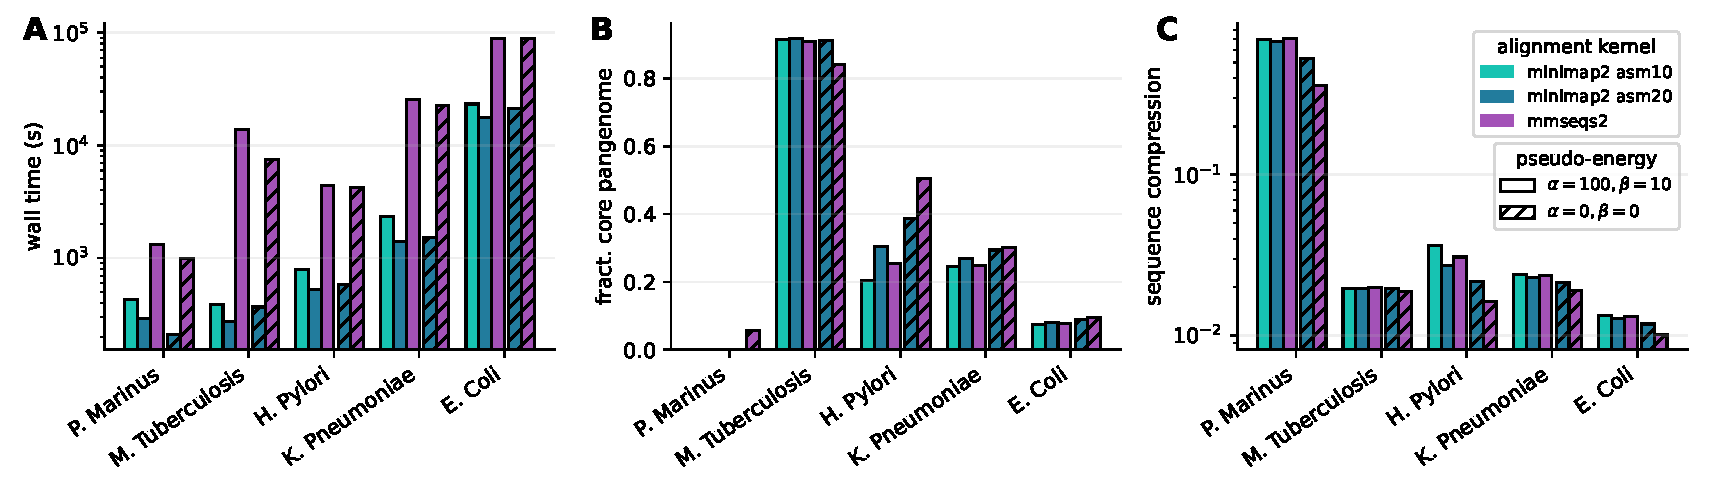
\includegraphics[width=.7\textwidth]{figs/panx_benchmark.pdf}
    \caption{{\bf Benchmark on real data}.}
    \label{fig:panx-benchmark}
\end{figure*}

The computational time and maximum memory required to build each alignment is summarized in Table \ref{table:panx-performance}.

\begin{table}[hb]
    \caption{{\bf Real-world Performance}.
        Elapsed time and maximum RAM usage needed to compute the pangraph for the following collections of RefSeq genomes.
        All runs were performed on an AMD Ryzen 7 2700X utilizing 8 cores.
    }
    \begin{tabular}{l r r r }
        \hline\hline
        Species         & Sample size & Wall time (min) & Max memory (GB) \\
        \hline
        E.~coli         & 307         & 426             & 11.7            \\
        H.~pylori       & 85          & 102             & 1.2             \\
        K.~pneumoniae   & 109         & 132             & 2.1             \\
        M.~tuberculosis & 51          & 91              & 0.4             \\
        P.~marinus      & 10          & 12              & 0.1             \\
        \hline
    \end{tabular}
    \label{table:panx-performance}
\end{table}

\begin{figure*}[htb]
    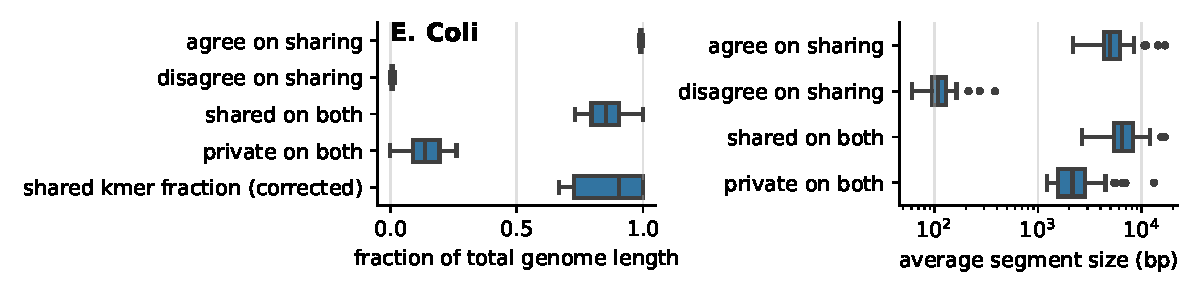
\includegraphics[width=.8\textwidth]{figs/proj_single_escherichia_coli.pdf}
    \caption{{\bf Test of graph marginalization}.}
    \label{fig:marginalization}
\end{figure*}

\section{Discussion}
While single nucleotide differences in the core genome are straightforward to analyze with existing tools, these analysis miss the great majority of genetic diversity.
The ability to rapidly align large sets of closely related, fully assembled genomes is a critical tool for the investigation of the processes governing microbial evolution.
We hope PanGraph will spur novel insight microbial diversity and the processes by which bacteria adapt and change.

Currently, PanGraph is limited to collections of genomes that are closely related with typical sequence divergence smaller that than 3\%.
This limitation originates from the core tool used for pairwise alignment, \texttt{minimap2}, that was determined to lose sensitivity if sequences are sufficiently diverged under the chosen parameters.
Homologous sequence that is more diverged than this cut-off will not be reliably merged by pangraph.
This effectively limits the TMRCA of sequences within a block.
More diverged sequence, for example originating from a cross-species transfer event, will thus be represented as alternative path.
In addition to the intrinsic limit of \texttt{minimap2}, this cut-off can be tuned with the parameter $\alpha$ and can for example be used to restrict merging to very similar sequences and thus capture all recent horizontal events as divergent paths in the graph.

We emphasize that PanGraph was designed as a modular tool.
In the future, we anticipate utilizing other pairwise ``alignment" kernels in addition to minimap2 that will allow the user to trade-off speed for sensitivity.

\section*{Acknowledgement}
We are grateful to Boris Shraiman for stimulating discussions.
This study was funded by the University of Basel and the NSF.

\bibliography{cite}{}

\end{document}